\documentclass[a4paper]{article}

% Packages.
\usepackage{amsthm}
\usepackage[answerdelayed]{exercise}
\usepackage[usenames,dvipsnames]{color}

% Definitions.
\theoremstyle{definition}
\newtheorem{definition}{Definition}

\renewcommand{\ExerciseHeader}{\vspace{7mm}\par\noindent\textbf{\large
\ExerciseName\ \ExerciseHeaderNB\ExerciseHeaderTitle
\ExerciseHeaderOrigin}\par}

\renewcommand{\AnswerHeader}{\par\noindent\textbf{
Answer of \ExerciseName\ \ExerciseHeaderNB}\par}

% Options.


\title{Student's $t$ test}
\author{Guillaume Filion}
\usepackage{Sweave}
\begin{document}
\maketitle


%% The problem %%
\section{The problem}

Do you pipette the same volume of liquid with a filter tip and a
normal tip? If anything, one would expect that you would pipette
a smaller volume with filter tips because the filter would hinder the
suction. Is that the case?

To answer that question I took my P200, pipetted 100 $\mu$L
of water 5 times with filter tips and 5 times with normal tips and
carefully weighed the water with a precision scale. Here is the data,
where the numbers represent the volume in $\mu$L.

\begin{Schunk}
\begin{Sinput}
> # Copy the data in your R session.
> filter_tips <- c(96.2, 99.0, 98.3, 98.0, 98.7);
> normal_tips <- c(96.6, 98.9, 97.9, 97.1, 97.7);
\end{Sinput}
\end{Schunk}

\begin{Exercise}
Together, formulate the problem in mathematical terms. How do we
approach the problem? What assumptions do we have to make? Discuss
their likelihood.
\end{Exercise}
\begin{Answer}
We need to formulate \textbf{a null hypothesis $H_0$}. In that
particular case, a good hypothesis is the following:
\begin{enumerate}
\item
Both datasets are sampled from a Gaussian distribution.
\item
\label{reject}
The parameters are unknown, but equal in both cases.
\item
Sampling is IID (\textbf{Independent} with Identical Distribution).
\end{enumerate}
In the alternative hypothesis item \ref{reject} is replaced by:
`The parameters are unknown, the standard deviations are equal
but the means are different.'
\end{Answer}


%% Statistical tests %%
\section{Statistical tests}

Intuitively, we would like to know if the observed difference of means
pipetted volume could occur at random. For this, we need to know more
about this `at random', and in particular, we need to know more about
the behaviour of the mean under the asumption of randomness.

The fundamental idea of statistical tests is to decide whether the
outcome of an experiment can be produced by sheer randomness. To
this end, every test has a \textbf{statistic} (note the absence of s
at the end) that measures an effect. The mean and the difference of
means between two samples are examples of statistics. Tests also have
a \textbf{null hypothesis} that allows to predict the distribution
of the statistic under the assumption of randomness. All tests also
have an alternative hypothesis, the one that will be accepted if the
null is rejected. Finally, tests
have a decision rule allowing to decide whether the null hypothesis
is accepted.


\begin{definition}[statistical test]
\label{test}
A statistical test is a protocol consisting of:
  \begin{enumerate}
  \item
  A null hypothesis.
  \item
  An alternative  hypothesis.
  \item
  A protocol to collect data.
  \item
  A test statistic.
  \item
  A decision rule.
  \end{enumerate}
\end{definition}

\begin{Exercise}
Together, discuss which are good and bad choices for these items,
either in general or for the proposed problem.
\end{Exercise}


%% Gaussian variables %%
\section{Gaussian variables}

We need to get a good view of the possible outcomes under the assumption
of randomness, \textit{i.e.} under the null hypothesis. For this, we
have to look into Gaussian variables.

The function \texttt {rnorm} is used to generate Gaussian random
variables. Each time you invoke it, you get a different result.
\begin{Schunk}
\begin{Sinput}
> rnorm(5); # Standard Gaussian sample.
\end{Sinput}
\begin{Soutput}
[1]  1.53692414 -0.29657556 -0.75560942 -0.53001983  0.01449643
\end{Soutput}
\begin{Sinput}
> rnorm(5); # Same input, different output.
\end{Sinput}
\begin{Soutput}
[1]  1.129708979  0.647003595  0.007945681  0.398744351 -1.208667672
\end{Soutput}
\begin{Sinput}
> rnorm(5, mean=1.5, sd=2.3);
\end{Sinput}
\begin{Soutput}
[1] -5.1059392  1.3714179  3.0780552  2.1063497 -0.8249848
\end{Soutput}
\end{Schunk}

We will make extensive use of \texttt{rnorm} in what follows.

\begin{Exercise}
Use the functions \texttt{mean} and \texttt{rnorm} to compute the
mean of a random sample of size 5 from a standard Gaussian variable.
Compute the difference between the means of two samples of size 5.
\end{Exercise}
\begin{Answer}
\begin{Schunk}
\begin{Sinput}
> mean(rnorm(5));
> mean(rnorm(5)) - mean(rnorm(5));
\end{Sinput}
\end{Schunk}
\end{Answer}


\begin{Exercise}
\label{genmean}
Now do the same 10,000 times to generate a sample of size 10,000
consisting of the difference of means of two standard Gausissan
samples of size 5. Store the result in a vector called
\texttt{diffmeans}.
\par\noindent\textcolor{Blue}{\textbf{Hint:} Use a \texttt{for} loop.}
\end{Exercise}
\begin{Answer}
\begin{Schunk}
\begin{Sinput}
> diffmeans <- rep(NA, 10000);
> for (i in 1:10000) {
+    diffmeans[i] <- mean(rnorm(5)) - mean(rnorm(5));
+ }
\end{Sinput}
\end{Schunk}
\end{Answer}

\begin{Exercise}
\label{sd}
Compute the standard deviation of a standard Gaussian random sample of
size 10, 100, 1000 and 10,000. What do you observe?
\end{Exercise}
\begin{Answer}
\begin{Schunk}
\begin{Sinput}
> sd(rnorm(10));
> sd(rnorm(100));
> sd(rnorm(1000));
> sd(rnorm(10000));
\end{Sinput}
\end{Schunk}
\par
The values converge to 1. This is the theoretical standard deviation
of a standard Gaussian random variable.
\end{Answer}

\begin{Exercise}
Compute the standard deviation of a subsample of size 10, 100, 1000 and
10,000 from the sample generated at exercise \ref{genmean}. What do you
observe?
\par\noindent\textcolor{Blue}{\textbf{Hint:} You can use the function
\texttt{sample}.}
\par\noindent\textcolor{BrickRed}{\textbf{For the aces:} To what
value do the numbers converge?}
\end{Exercise}
\begin{Answer}
\begin{Schunk}
\begin{Sinput}
> sd(sample(diffmeans, size=10));
> sd(sample(diffmeans, size=100));
> sd(sample(diffmeans, size=1000));
> sd(sample(diffmeans, size=10000));
\end{Sinput}
\end{Schunk}
\par
The values converge to some number smaller than 1. You can check that
it is close to $\sqrt{2/5}$.
\end{Answer}

\begin{Exercise}
Plot the density of a random sample of size 10,000 from a standard
Gaussian random variable. Plot the density of the sample generated
at exercise \ref{genmean} (\texttt{diffmeans})
on the same graph. What do you observe?
\par\noindent\textcolor{Blue}{\textbf{Hint:} \texttt{plot(density(...))}
 and \texttt{lines(density(...))} will help.}
\end{Exercise}
\begin{Answer}
\begin{Schunk}
\begin{Sinput}
> plot(density(diffmeans), main="Density plots", xlab="Value");
> lines(density(rnorm(10000)), col="red");
> legend(x="topleft", lwd = 1, col=c("black", "red"),
+    legend=c("Diff. means", "Std Gaussian"));
\end{Sinput}
\end{Schunk}
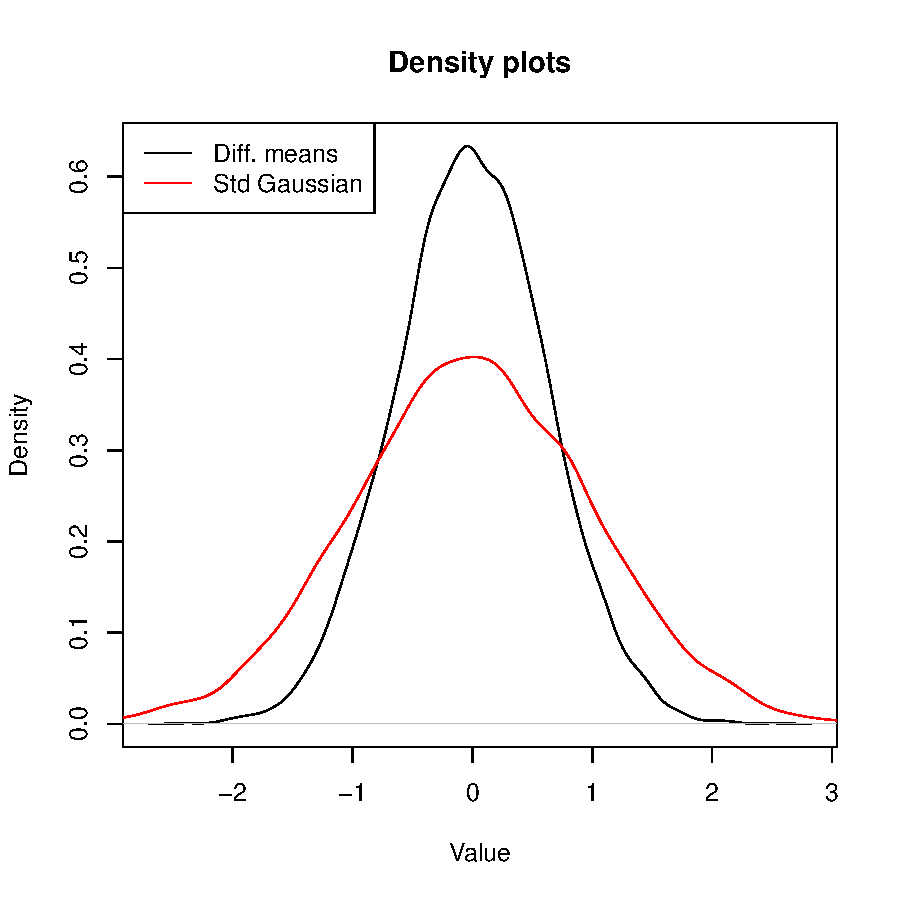
\includegraphics{ttest-007}
\par
Both density plots have the same shape. Actually, they are both
Gaussian, but the density of differences of means has smaller
standard deviation, as shown by the fact that it is narrower.
\end{Answer}

\begin{Exercise}
Compute the standard deviations of samples of size 10,000 consisting
of the differences of averages of sample of sizes 5 and 5, 50 and 50,
500 and 500, 5,000 and 5,000 from standard Gaussian random
variables. What do you observe?
\end{Exercise}
\begin{Answer}
\begin{Schunk}
\begin{Sinput}
> samples <- list();
> for (i in c(5, 50, 500, 5000)) {
+    for (j in 1:10000) {
+       samples[[as.character(i)]][j] <- mean(rnorm(i))-mean(rnorm(i));
+    }
+ }
> lapply(samples, sd);
\end{Sinput}
\end{Schunk}
\par
The standard deviation converges to 0. It has to be clear for you
that the standard deviation of a Gaussian random sample does
\textbf{not} converge to 0 as the sample size increases. It is
\textbf{the standard deviation of the estimated mean}, or the
\textbf{standard deviation of the difference of estimated means}
that converges to 0. The estimate of the difference of means is more
and more accurate as the sample size increases.
\end{Answer}


%% Estimating the standard deviation %%
\section{Estimating the standard deviation}

The estimated standard deviation of a sample $(x_1, x_2, ..., x_n)$,
as computed by the function \texttt{sd} is defined by the formula:

\begin{equation}
  S = \sqrt{\frac{1}{n-1}\sum_{i=1}^n(x_i-\bar{x})^2}, \mbox{ where }
    \bar{x} = \frac{1}{n}\sum_{i=1}^n x_i.
\end{equation}

This value is an estimator of the true standard deviation, and is itself
subject to random variation, as shown in exercise \ref{sd}. For large
samples, this value will be close to expected, but for small samples
it can be far off-target.

\begin{Exercise}
\label{var}
Assume independent sampling of $(x_1, ..., x_n)$ from a distribution
with standard deviation $\sigma$. What is the standard deviation of the
estimated sample mean? Suggest an estimator for the standard deviation
of the mean of a sample.
\par\noindent\textcolor{Blue}{\textbf{Hint:} Recall that
$Var(aX) = a^2 Var(X)$. Besides, if $X$ and $Y$ are independent,
$Var(X+Y) = Var(X) + Var(Y)$.}
\end{Exercise}
\begin{Answer}
The variance of the distribution is $\sigma^2$. The variance of $x_i/n$
is $\sigma^2/n^2$ Because of independence, the variance of
$x_1/n + ...  + x_n/n$ is $n\sigma^2/n^2 = \sigma^2/n$, which is
the variance of the estimated mean. The standard deviation is found
by taking the square root: $\sqrt{\sigma^2/n} = \sigma/\sqrt{n}$.
\par
Based on this result, the natural estimator for the standard deviation
of the mean of a sample comes as:
\begin{equation}
  \frac{S}{\sqrt{n}} = \sqrt{\frac{1}{n(n-1)}\sum_{i=1}^n
    (x_i-\bar{x})^2}.
\end{equation}
\end{Answer}

\begin{Exercise}
Generate 10,000 standard Gaussian random samples of size 5 and
computre their estimated standard deviations. Plot the histogram of
these estimated standard deviations. Does this look Gaussian?
\par\noindent\textcolor{Blue}{\textbf{Hint:} Take inspiration from
exercise \ref{genmean} to generate the sample, and use \texttt{hist}.}
\end{Exercise}
\begin{Answer}
\begin{Schunk}
\begin{Sinput}
> stddevs <- rep(NA, 10000);
> for (i in 1:10000) {
+    stddevs[i] <- sd(rnorm(5));
+ }
> hist(stddevs, main="Histogram of the estimated standard deviation",
+    xlab="Value");
\end{Sinput}
\end{Schunk}
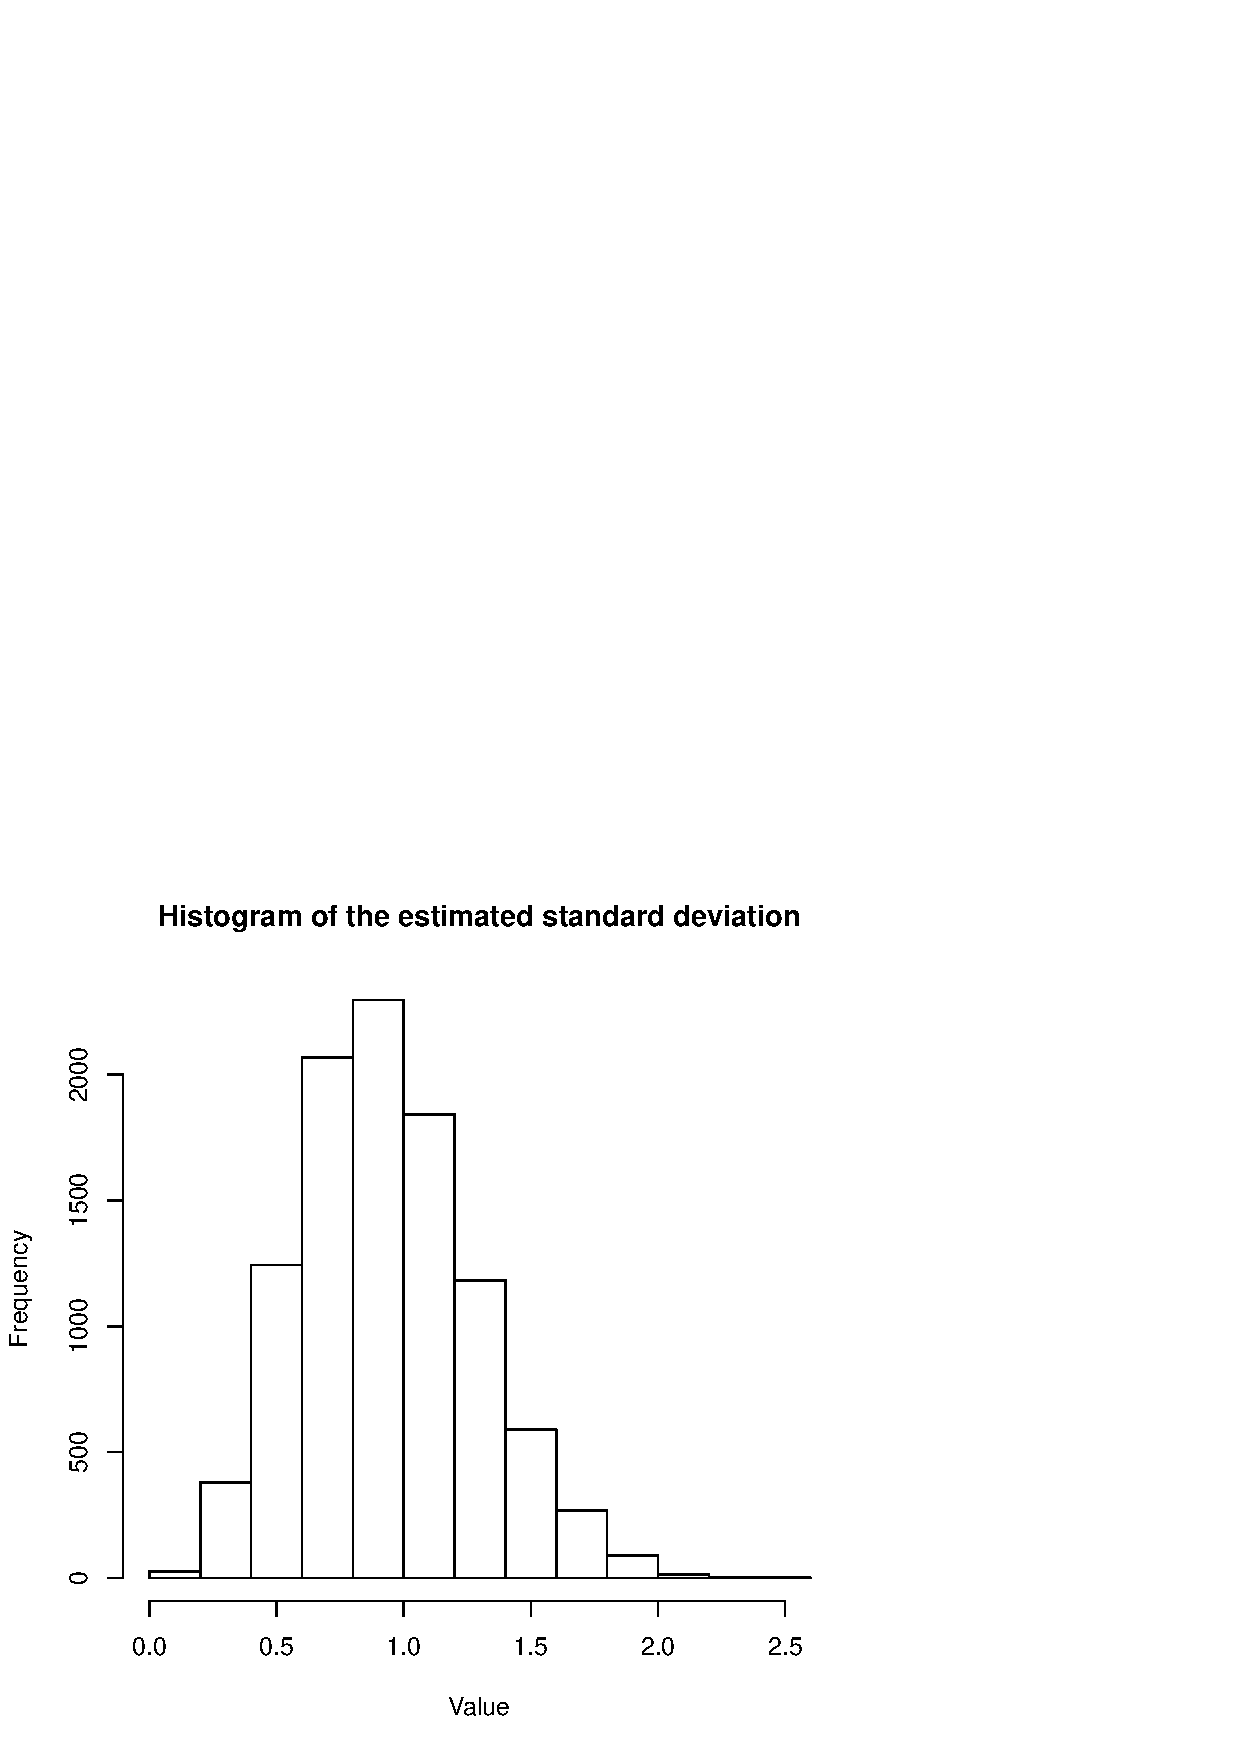
\includegraphics{ttest-009}
\par
The distribution of the estimated standard deviation is not Gaussian.
Because the standard deviation is always positive the distribution is
not symmetric.
\end{Answer}


%% Effect size %%
\section{Effect size}

We are confronted with the difficulty of estimating the distribution
of the mean with an imprecise value of the standard deviation.

\begin{Exercise}
Together, suggest a way to go around this difficulty. If estimating
two parameters at the same time is too difficult, isn't there a way to
work with a single number?
\end{Exercise}
\begin{Answer}
As suggested by the title of this section. We can work with the
\textbf{effect size}, \textit{i.e.} the mean divided by the standard
deviation of the mean.
\end{Answer}

\begin{Exercise}
Generate 10,000 standard Gaussian samples of size 5 and compute their
effect size. Plot the density of their distribution. Is it Gaussian?
\end{Exercise}
\begin{Answer}
\begin{Schunk}
\begin{Sinput}
> esize <- rep(NA, 10000);
> for (i in 1:10000) {
+    Gaussian.sample <- rnorm(5);
+    esize[i] <- sqrt(5)*mean(Gaussian.sample)/sd(Gaussian.sample);
+ }
> plot(density(esize), xlab="Value", main="Density of effect size");
> lines(density(rnorm(10000, mean(esize), sd(esize))), col="red");
> legend(x="topleft", lwd = 1, col=c("black", "red"),
+    legend=c("Effect size", "Gaussian"));
\end{Sinput}
\end{Schunk}
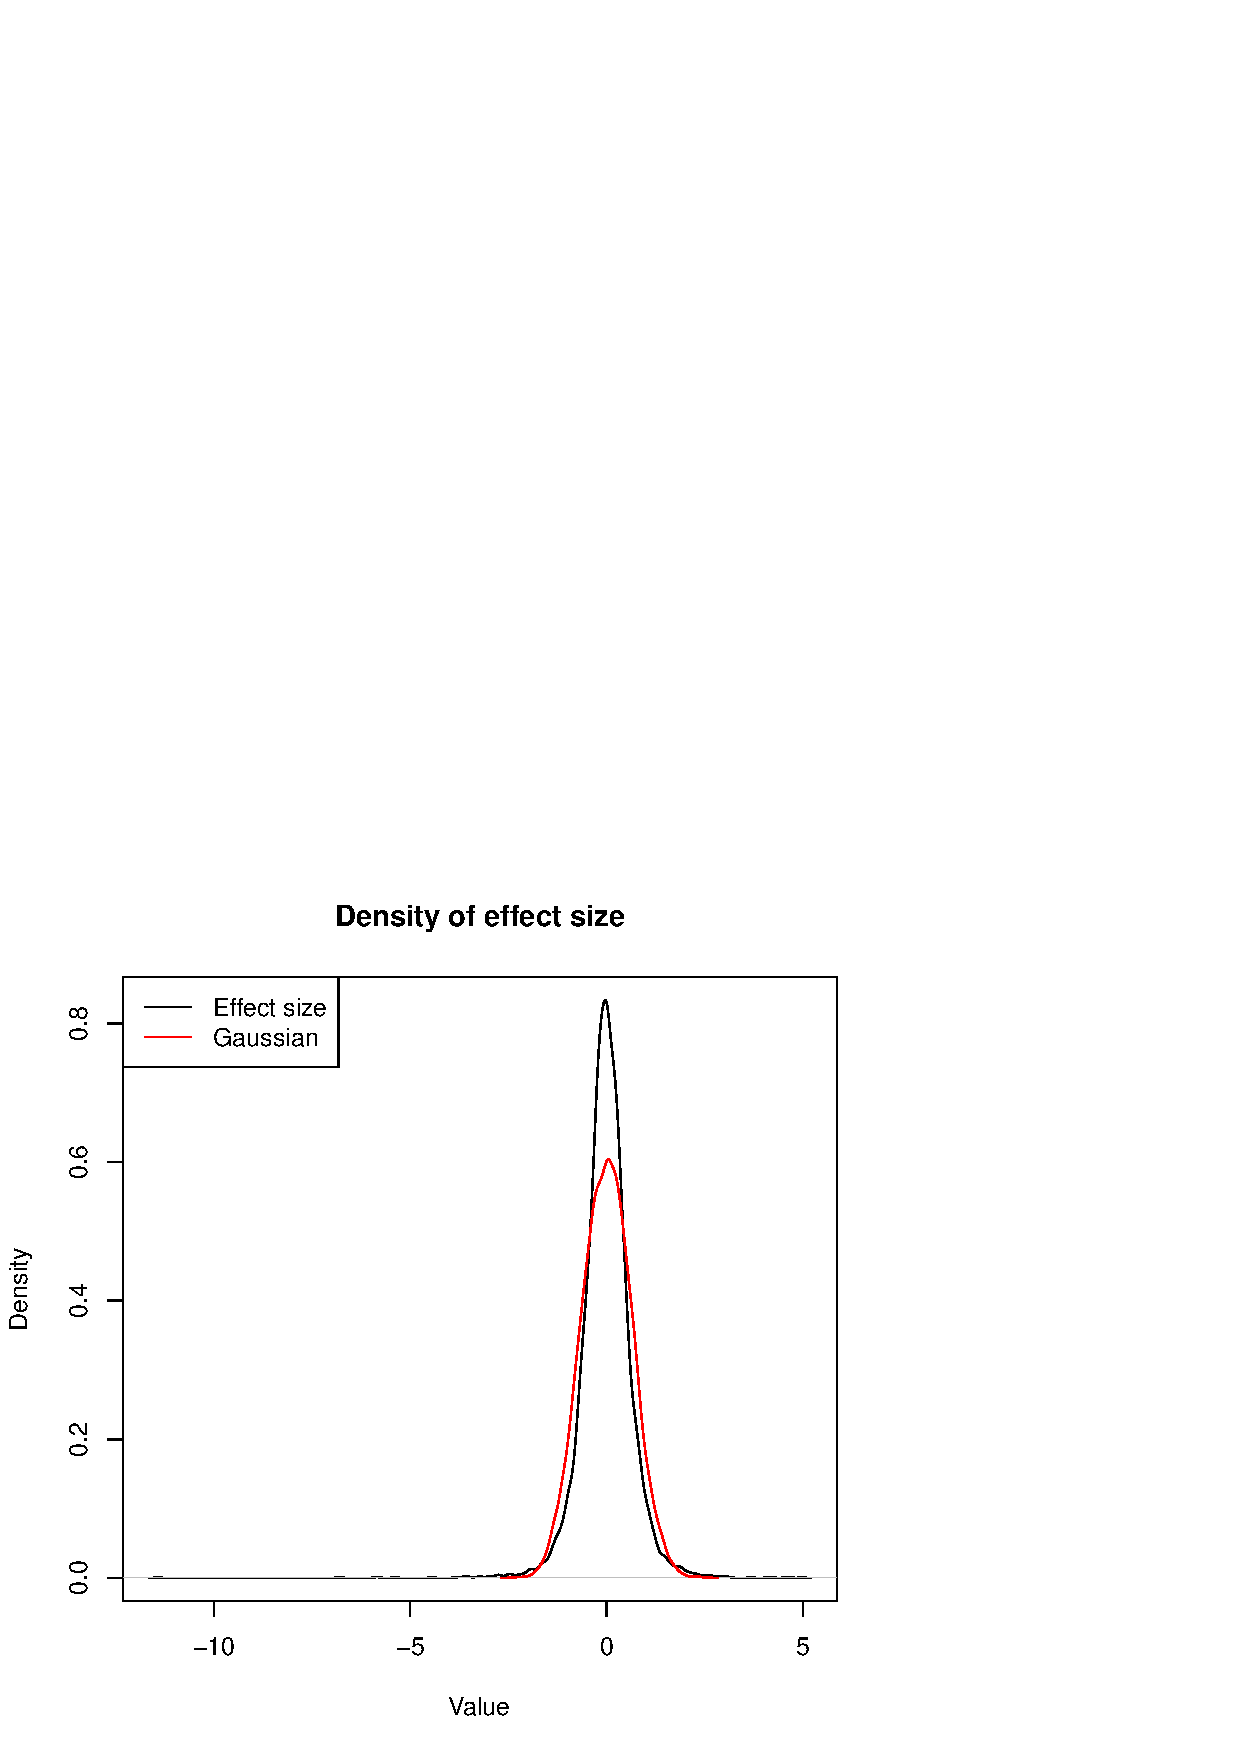
\includegraphics{ttest-010}
\par
The distribution is symmetric and bell-shaped but it is not Gaussian.
The red line on the previous graph is the density of the distribution
of a Gaussian variable with same mean an standard deviation as the
effect size. The distribution of the effect size has so called
`heavy tails', which are usually visible
because of the presence of outliers far off the bulk of values around
0. The outliers occur in samples where all 5 values are close to each
other, which gives a very small estimated standard deviation and
therefore an inflated effect size ratio.
\end{Answer}

\begin{Exercise}
\label{efsize}
In the case of two samples $(x_1, ..., x_n)$ and $(y_1, ..., y_n)$
sampled from a distribution with the same standard deviation, what
is the effect size for the difference of means?
\par\noindent\textcolor{Blue}{\textbf{Hint:} What is the variance
of the mean? What are the variance and standard deviation of the
difference of means?}
\par\noindent\textcolor{BrickRed}{\textbf{For the aces:} Can you
compute the effect size if the samples have different sizes?}
\end{Exercise}
\begin{Answer}
Denote $S^2_x$ and $S^2_y$ the estimated variances of the first
and second samples respectively. The estimated variances of the
means are $S^2_x/n$ and $S^2_y/n$, so that the estimated
variance of the difference is $S^2_x/n+S^2_y/n$ (see hint of
exercise \ref{var}), and the estimated standard deviation
$\sqrt{(S^2_x+S^2_y)/n}$. The effect size is thus

\begin{equation}
  \frac{\sqrt{n}(\bar{x} - \bar{y})}{\sqrt{S_x^2 + S_y^2}}.
\end{equation}
\end{Answer}

\begin{Exercise}
Suppose $(x_1, ..., x_n)$ and $(y_1, ..., y_n)$ are sampled from
the same population with mean 0 and variance 1. Let's transform
the samples by adding a constant $a$, \textit{i.e.}
$\tilde{x}_i = x_i + a$ and $\tilde{y}_i = y_i + a$. How does
this change the effect size? Let's further transform the sample
by multiplying the values by a constant $b$, \textit{i.e.}
$\mathring{x}_i = b\tilde{x}_i$ and $\mathring{y}_i = b\tilde{y}_i$.
How is the effect size changed this time?
\par\noindent\textcolor{Blue}{\textbf{Hint:} Remember that the
variance (or estimated variance) of $X + a$ is the variance (or
estimated variance) of $X$}.
\end{Exercise}
\begin{Answer}
$\bar{\tilde{x}} = \bar{x} + a$ and $\bar{\tilde{y}} = \bar{y} + a$.
According to the hint, $S^2_{\tilde{x}} = S^2_x$ and
$S^2_{\tilde{y}} = S^2_y$. So adding a constant does not change the
effect size.
\par
$\bar{\mathring{x}} = b\bar{x} + ab$ and $\bar{\mathring{y}} = b\bar{y} + ab$.
$S^2_{\mathring{x}} = b^2S^2_x$ and $S^2_{\mathring{y}} = b^2S^2_y$.
The $b$'s in the numerator and denominator cancel out, so multiplying by
a constant also does not change the effect size.
\end{Answer}

\section{The null hypothesis}

We now have a statistic for the test with a very useful property:
\textbf{it is invariant by shifting and scaling}.
This means that we can study the effect size on a standard Gaussian
distribution with mean 0 and variance 1. All the Gaussian distributions
are obtained by shifting and scaling the standard Gaussian, so the
distribution of the effect size computed from any Gaussian distribution
will be exactly the same as the distribution of the effect size
computed from the standard Gaussian.

Let's make sure of that, and see what happens when the null hypothesis
is not true.

\begin{Exercise}
\label{genefsize}
Generate a random sample of size 10,000 consisting of the effect
size designed in exercise \ref{efsize} for two standard Gaussian
samples of size 5. Store the result in a vector called \texttt{esize}.
\end{Exercise}
\begin{Answer}
\begin{Schunk}
\begin{Sinput}
> esize <- rep(NA, 10000);
> for (i in 1:10000) {
+    x <- rnorm(5);
+    y <- rnorm(5);
+    esize[i] <- sqrt(5)*(mean(x)-mean(y))/sqrt(var(x)+var(y));
+ }
\end{Sinput}
\end{Schunk}
\end{Answer}

\begin{Exercise}
Repeat the task of exercise \ref{genefsize} with other Gaussian
random variables \textit{i.e.} change the \texttt{mean} and
\texttt{sd} parameters of \texttt{rnorm}, but keep the parameters
equal for both samples (\textit{i.e.} assume that the null
hypothesis is true). Overlay the obtained densities of the effect
size with the one obtained for the standard Gaussian.
\par\noindent\textcolor{BrickRed}{\textbf{For the aces:} Use
different parameters for both populations (\textit{i.e.} assume
that the null hypothesis is false).}
\par\noindent\textbf{Note:} Keep a sample size of 5.
\end{Exercise}

%% The decision rule %%
\section{The decision rule}

We have almost everything. We just need to find a decision rule that makes
sense. Several criteria have been proposed by different statistical schools.
We will use the widespread frequentist approach.

The frequentist approach is to choose a level of risk, usually called
$\alpha$, that is the probability of rejecting the null hypothesis,
given that it is actually true. The most commonly encoutered values for
$\alpha$ are 0.05 and 0.01, but both are abitrary (there is no particular
reason why these values are better than others). Based on that, we
delineate a \textbf{rejection region} at level $\alpha$, \textit{i.e.}
a set of statistic values that has a probability of occurrence equal
to $\alpha$ if the null hypothesis is true.

\begin{definition}[level of a test]
The level of a test is the probability of rejecting the null
hypothesis given that it is true.
\end{definition}

\begin{Exercise}
\label{thresh}
Set $\alpha = 0.05$. What is the most meaningful rejection region for
the effect size? Give a numerical estimate of that region.
\par\noindent\textcolor{Blue}{\textbf{Hint:} Use the results of
exercise \ref{genefsize}.}
\end{Exercise}
\begin{Answer}
There is a matter of discussion whether this is a unilateral of bilateral
test. Bear in mind that unilateral tests make a very strong assumption,
in that case, that it is strictly physically \textbf{impossible} that
you pipette more volume with filter tips, and that even if you measured
a volume 10 times bigger with filter tips, you would accept the null
hypothesis (thereby coming to the conclusion that there is no difference
in the volume you pipette). For this kind of test, only extraordinary
circumstances would call for unilateral testing. Therefore a symmetric
rejection region, distant from the bulk of the values around 0
is the most meaningful.
\par
The limits of that region can be estimated from the distribution
of the effect size.
\begin{Schunk}
\begin{Sinput}
> abs_threshold <- quantile(abs(esize), probs=0.95);
> abs_threshold;
\end{Sinput}
\begin{Soutput}
    95% 
2.26078 
\end{Soutput}
\begin{Sinput}
> quantile(esize, probs=c(0.025, 0.975)); # is not symmetric.
\end{Sinput}
\begin{Soutput}
     2.5%     97.5% 
-2.294104  2.233898 
\end{Soutput}
\end{Schunk}
\end{Answer}

\begin{Exercise}
Compute the effect size from the measurements and store the result in a
vector called \texttt{t}. Apply the decision rule
and conclude whether or not to accept the null hypothesis.
\end{Exercise}
\begin{Answer}
\begin{Schunk}
\begin{Sinput}
> t <- sqrt(5) * (mean(filter_tips) - mean(normal_tips)) /
+    sqrt(var(normal_tips) + var(filter_tips));
> print(t);
\end{Sinput}
\begin{Soutput}
[1] 0.6387136
\end{Soutput}
\begin{Sinput}
> mean(abs(esize) > abs(t));
\end{Sinput}
\begin{Soutput}
[1] 0.5354
\end{Soutput}
\end{Schunk}
\par
The computed effect size does not fall in the rejection region.
We accept the null hypothesis and conclude that you pipette the same
volume with filter tips and normal tips.
\end{Answer}


%% The p-value %%
\section{The p-value}

You may have noticed that the p-value is not an ingredient of a statistical
test (see definition \ref{test}). The conclusion of a statistical test
is always to accept or reject the null hypothesis, never to be in doubt,
borderline significant, call for more data or let the readers judge by
themselves. In that sense, true statistical tests are a rarity of
scientific litterature.

The idea of the p-value is to let the audience judge by themselves if
a test should be rejected or not. If two statisticians work at different
levels $\alpha$, there is no reason why one should impose her conclusions
on the other. The introduction of the p-value of a test came with the advent
of computers. When only statistical tables were available, it was tedious
to compute it and therefore accepted to use the level $\alpha$ as a
reference.

By definition, the p-value of a test is the probability of observing
a larger test statistic than the one you measured, assuming that the null
hypothesis is true. Here, `larger' is usually defined by the context.
For example, in the case of the $t$ test designed previously, it means
`larger in absolute value'.

\begin{Exercise}
Suppose that a test has a statistic $\theta$, and that the rejection
region is always of the form $\theta > s(\alpha)$, where the threshold
depends on the level $\alpha$.
If the p-value of the test is 0.03, what does that mean for the decision
rule at level 0.05 and 0.01? What is the largest 
level $\alpha$ for which the null hypothesis would be accepted?
\end{Exercise}
\begin{Answer}
Suppose that the observed value of $\theta$ is $\theta_0$. By definition
$P(\theta > \theta_0) = 0.03$. Note that $P(\theta > s(0.05)) = 0.05$,
which is possible only if $\theta_0 > s(0.05)$, \textit{i.e.} the null
hypothesis is rejected at level 0.05. Symmetrically,
$P(\theta > s(0.01)) = 0.01$, so we must have $\theta_0 < s(0.01)$ and the
null hypothesis is accepted at level 0.01.

If we had chosen the largest level $\alpha$ for which the null hypothesis
would be accepted, observing any larger $\theta$ would involve rejecting
the null hypothesis at level $\alpha$. So $P(\theta > \theta_0) = \alpha$.
But we know that this value is 0.03, the p-value of the test. This gives
rise to an alternative definition of the p-value of a test as \textbf{the
largest level $\alpha$ for which the null hypothesis is accepted
for this value of the statistic}.
\end{Answer}

\begin{Exercise}
Give an estimate of the p-value of the test.
\par\noindent\textcolor{Blue}{\textbf{Hint:} Use the results of
exercise \ref{genefsize}.}
\end{Exercise}

\begin{Exercise}
The \texttt{R} command to perform a $t$ test is \texttt{t.test}.
Use it to test the null hypothesis and compare the results with
the ones you obtained previously.
\par\noindent\textcolor{Blue}{\textbf{Hint:} Don't forget to check
\texttt{?t.test} or \texttt{help(t.test)} if in doubt.}
\end{Exercise}
\begin{Answer}
\begin{Schunk}
\begin{Sinput}
> t.test(filter_tips, normal_tips);
\end{Sinput}
\begin{Soutput}
	Welch Two Sample t-test

data:  filter_tips and normal_tips 
t = 0.6387, df = 7.608, p-value = 0.5418
alternative hypothesis: true difference in means is not equal to 0 
95 percent confidence interval:
 -1.057203  1.857203 
sample estimates:
mean of x mean of y 
    98.04     97.64 
\end{Soutput}
\end{Schunk}
\end{Answer}


%% Power of the test %%
\section{Power of the test}

We have seen how statistical tests work if the null hypothesis is true.
But what if the null hypothesis is false? Well, if there is a risk
$\alpha$, one might expect that there also exists a risk $\beta$, and
that is the probability of accepting the null hypothesis given that
it is false.

The level $\alpha$ is always easy to know, or at least to approximate,
but the risk $\beta$ is a lot more difficult to control. Indeed,
there is usually one way the null hypothesis can be true, and infinitely
many ways it can be false. So the risk $\beta$ always depends on
\textbf{how} the null hypothesis is false.

For this reason, there is not a single risk $\beta$ associated with a
statistical test, but many. Actually the power of a test is not a
number, but a function.

\begin{definition}[power of a test]
The power of a statistical test is a function of hypotheses. It is
the probability of rejecting the null hypothesis given that this
particular hypothesis is true.
\end{definition}

\begin{Exercise}
Say that a test has power $W$, function of hypotheses denoted $H$.
What is $W(H_0)$? What does that tell you?
\end{Exercise}
\begin{Answer}
By definition, it is the probability of rejecting the null hypothesis
given that the null hypothesis is true, that is $\alpha$. This shows
that \textbf{The power of a test always depends on the risk $\alpha$}.
\end{Answer}

\begin{Exercise}
Call $\Delta$ the difference of volume between filter tips and normal
tips. Estimate the power of the test for $\Delta = 1 \mu$L, $5 \mu$L,
and $10 \mu$L. To this end, generate random samples of 10,000 values
of the effect size computed from two Gaussian samples of size 5, one
with a mean of 100, the other with a mean of $100 - \Delta$. Use
the estimate of the standard deviation from the data.
\par\noindent\textcolor{Blue}{\textbf{Hint:} Use the threshold
of the rejection region determined at exercise \ref{thresh}.}
\end{Exercise}
\begin{Answer}
\begin{Schunk}
\begin{Sinput}
> sdest <- sqrt((var(normal_tips) + var(filter_tips) / 2));
> W <- list();
> for (delta in c(1,5,10)) {
+    for (i in 1:10000) {
+       filter_t <- rnorm(5, mean=100-delta, sd=sdest);
+       normal_t <- rnorm(5, mean=100, sd=sdest);
+       W[[as.character(delta)]][i] <- sqrt(5) *
+          (mean(filter_t) - mean(normal_t)) /
+          (sqrt(var(filter_t) + var(filter_t)));
+    }
+ }
> for (x in W) {
+    print(mean(abs(x) > abs_threshold));
+ }
\end{Sinput}
\begin{Soutput}
[1] 0.2737
[1] 0.9998
[1] 1
\end{Soutput}
\end{Schunk}
\end{Answer}

\section{Robustness, exactness}

The power of a statistical test says whether it has good chances to
detect small effects \textit{i.e.} small effet sizes in our case.
Robustness is another property that is much more loosely defined.
A test is said to be robust relative to a particular hypothesis if
the value of the test statistic does not vary much if this
hypothesis is violated. Whether a test is robust depends on your
degree of tolerance, and also on how the hypothesis is violated.

An exact test gives an exact distribution of its statistic (if the
null hypothesis is true). If a test is not exact, it is approximate.

\begin{Exercise}
Is the $t$ test exact? Suppose that the variables are not prefectly
Gaussian. Is the $t$ test still exact?
\end{Exercise}
\begin{Answer}
Yes. No.
\end{Answer}

\begin{Exercise}
We will see whether the $t$ test is robust to the assumption of
normality. For this we will use exponential variables, generated
by \texttt{rexp}. You can check that the distribution of these
variables is far from Gaussian. Replace Gaussian by exponential
variables in the generation of a sample of the effect size
(\texttt{esize}) and compare the two distributions by overlaying
their density.
\end{Exercise}
\begin{Answer}
\begin{Schunk}
\begin{Sinput}
> esize_exp <- rep(NA, 10000);
> for (i in 1:10000) {
+    x <- rexp(5);
+    y <- rexp(5);
+    esize_exp[i] <- sqrt(5) * (mean(x) - mean(y)) /
+       (sqrt(var(x) + var(y)));
+ }
> plot(density(esize), main="Density plots", xlab="Value");
> lines(density(esize_exp), col="red");
> legend(x="topleft", lwd = 1, col=c("black", "red"),
+    legend=c("Gaussian", "Exponential"));
\end{Sinput}
\end{Schunk}
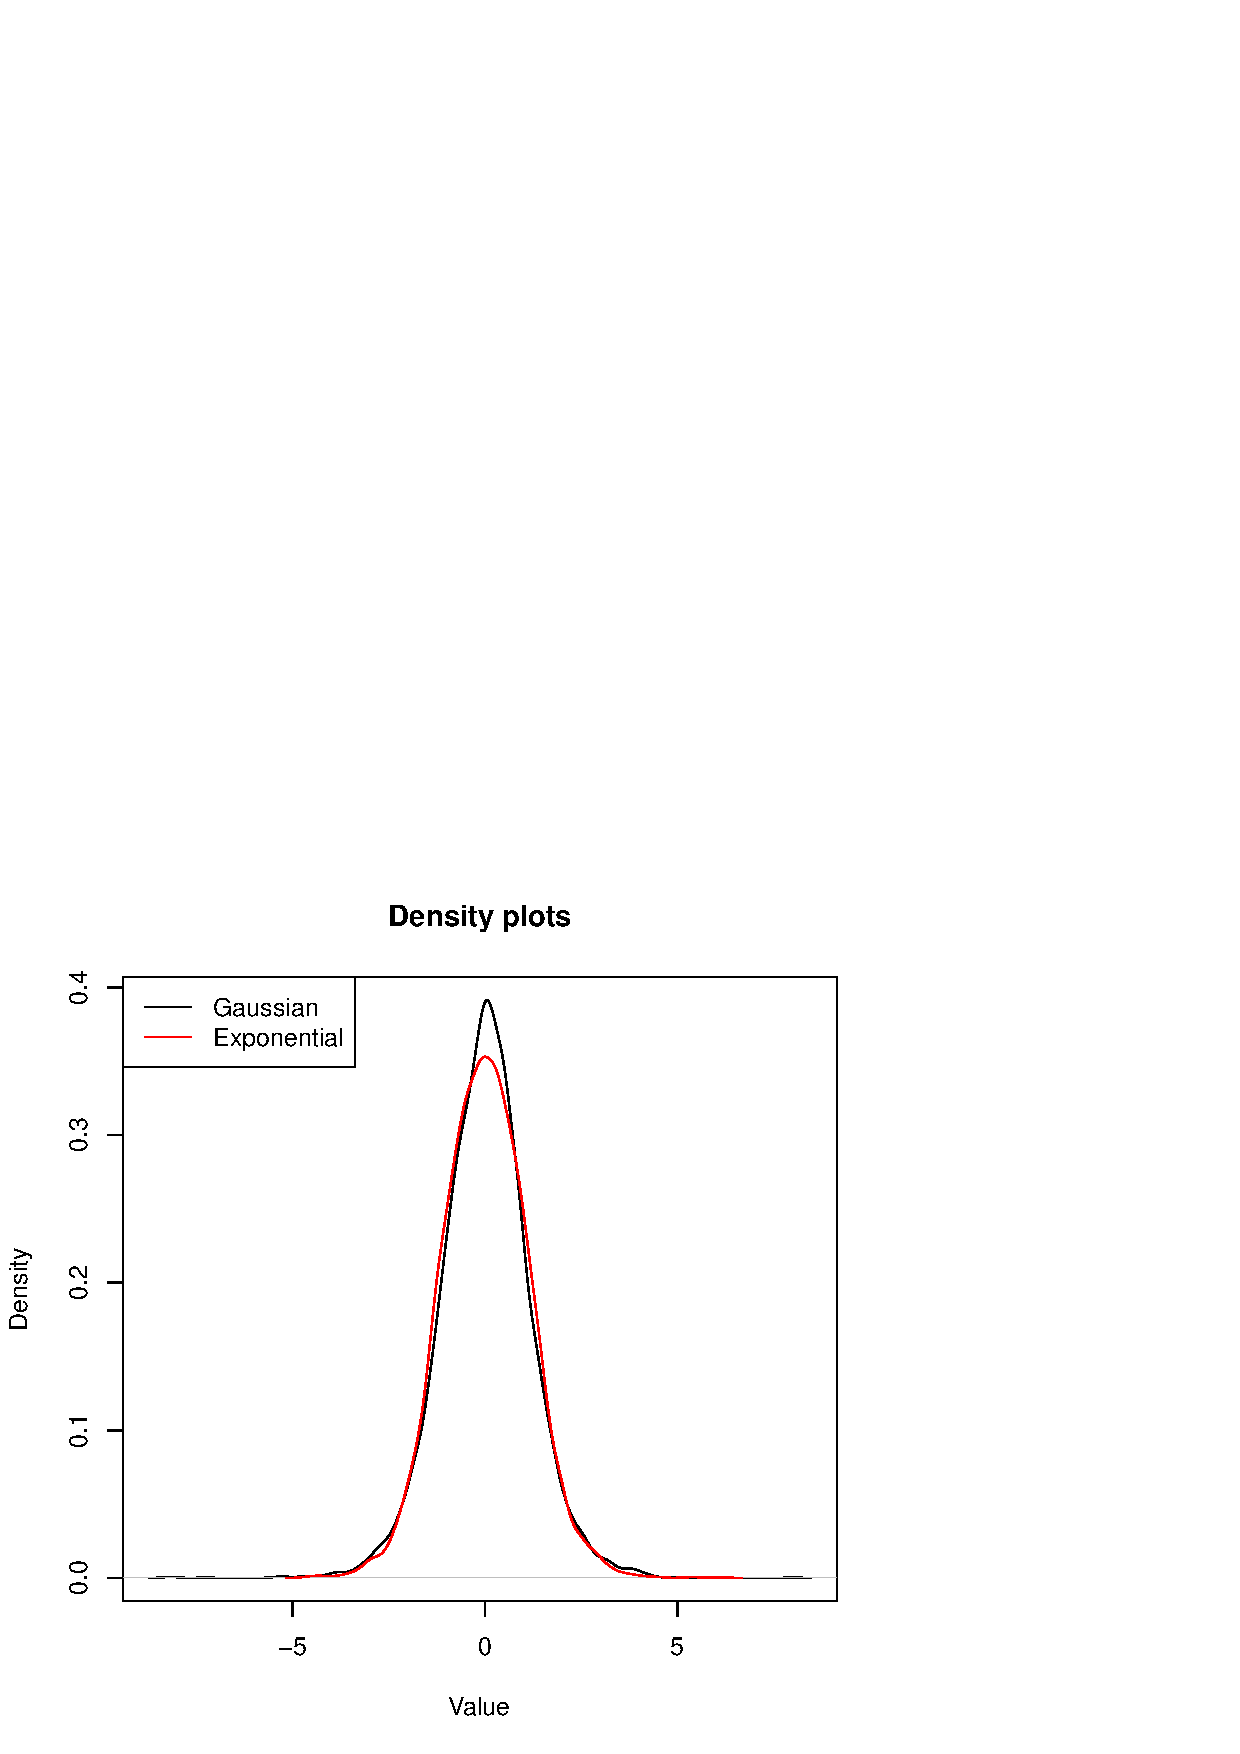
\includegraphics{ttest-016}
\par
The $t$ test is relatively robust to the departure from normality
because of the \textbf{Central Limit Theorem}. The theorem says
that the average of independently sampled variables becomes
progressively Gaussian as the sample size increases. A rule of
thumb is that for $n>30$, the approximation is good enough.
\end{Answer}

\cleardoublepage
\shipoutAnswer
\end{document}

